\documentclass{ctexbeamer}

\usetheme{Berkeley}

\title{Distributed Filesystem}

\author{曹隽诚 \and 李晋}
\date{2022年11月9日}

\begin{document}
\frame{\titlepage}

\section{Introduction}

\begin{frame}
\frametitle{Distributed Filesystem}
\framesubtitle{NFS}
\begin{exampleblock}{NFS}
  mount -t nfs master:/mnt /mnt
\end{exampleblock}
\begin{alertblock}{Distributed or just Remote}
  NFS is a remote filesystem, not necessarily a distributed one
\end{alertblock}
\begin{quotation}
  NFS does not support aggregating the storage resources on multiple systems into a virtual storage pool, instead it only allows accessing remote sotrage resources in a transparent way.
\end{quotation}
\end{frame}

\begin{frame}
\frametitle{Distributed Filesystem}
\framesubtitle{GlusterFS}
\begin{exampleblock}{GlusterFS}
  gluster volume create gv replica 2 node0:/data node1:/data
\end{exampleblock}
\begin{quotation}
  Just like on NFS, we see an identical filesystem tree on all participating nodes, but unlike on NFS where all files are located on master, they are distributed or replicated among all nodes.
\end{quotation}
\end{frame}

\section{Design}
\begin{frame}
\frametitle{Distributed Filesystem}
\framesubtitle{Communication}
\begin{block}{Requirement}
  A reliable transport for supporting a distributed filesystem
\end{block}
\begin{exampleblock}{Choices}
  \begin{itemize}
    \item stream
    \item message
    \item RMA (Remote \emph{Memory} Access)
  \end{itemize}
\end{exampleblock}
\end{frame}

\begin{frame}
\frametitle{Distributed Filesystem}
\framesubtitle{Communication}
\begin{verse}
  Do not communicate by sharing memory; instead, share memory by communicating.
\end{verse}
\begin{block}{stream}
  Explicit connections and states
\end{block}
\begin{block}{message}
  Asynchronous and full of callbacks
\end{block}
\begin{exampleblock}{RMA}
  RDMA with an optional D
\end{exampleblock}
\end{frame}

\begin{frame}[fragile]
\frametitle{Distributed Filesystem}
\framesubtitle{RMA}
  \begin{exampleblock}{RMA}
    Effective to implement on modern infrastructures with RDMA \\
    Gracefully fallbacks to stream or message without code change \\
    Naturally maps to NVME-like storage technologies \\
  \end{exampleblock}
  \begin{block}{Addressing}
    \begin{small}
    \begin{verbatim}
    0         63         127
    | node id | block id | \end{verbatim}
    \end{small}
  \end{block}
  \begin{block}{Operation}
    \begin{itemize}
       \item read
       \item write 
       \item discard
    \end{itemize}
  \end{block}
\end{frame}

\begin{frame}
\frametitle{Distributed Filesystem}
\framesubtitle{Filesystem}
  \begin{exampleblock}{RMA}
    Effectively, a distributed virtual block device \\
    Simply, run an existing filesytem atop
  \end{exampleblock}
  \begin{alertblock}{Locality}
    Normal filesystems have no idea of the distributed natual of the underlying block device, resulting in poor locality and poor performance
  \end{alertblock}
  \begin{block}{Bottomline}
    Preferably allocate blocks where they are created
  \end{block}
\end{frame}

\section{Impl}
\begin{frame}
\frametitle{Distributed Filesystem}
\framesubtitle{Filesystem}
\begin{verse}
  A Tale of Two Traits
\end{verse}
\begin{block}{rcore\_fs::vfs::FileSystem}
  Allows a single filesystem implementation to be used in rCore, zCore and fuse
\end{block}
\begin{block}{rcore\_fs\_dfs::transport::Transport}
  Allows the distributed filesystem to function reguardless of the underlying network and storage implementation
\end{block}
\end{frame}

\begin{frame}
\frametitle{Distributed Filesystem}
\framesubtitle{Transport}
\begin{block}{FUSE}
  rcore\_fs\_dfs::transport::loopback::LoopbackTransport \\
  point-to-point RPC-style TCP transport \\
\end{block}
\begin{block}{zCore}
  linux\_object::net::DistriTran \\
  Broadcast TCP transport with rendezvous point \\
\end{block}
\end{frame}

\begin{frame}
\frametitle{Distributed Filesystem}
\framesubtitle{Topology}
\begin{figure}
  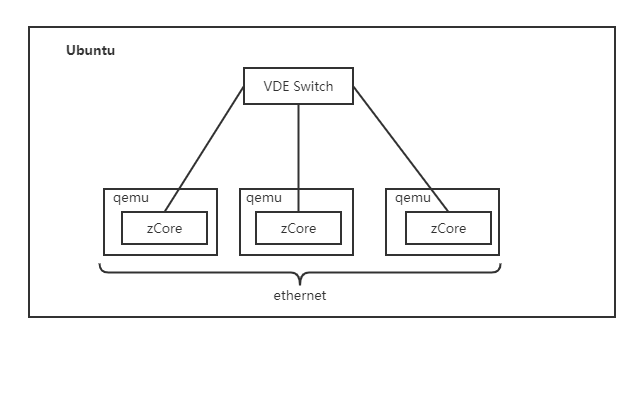
\includegraphics[width=\textwidth]{./images/image2.png}
\end{figure}
\end{frame}

\begin{frame}
\frametitle{Distributed Filesystem}
\framesubtitle{Topology}
\begin{figure}
  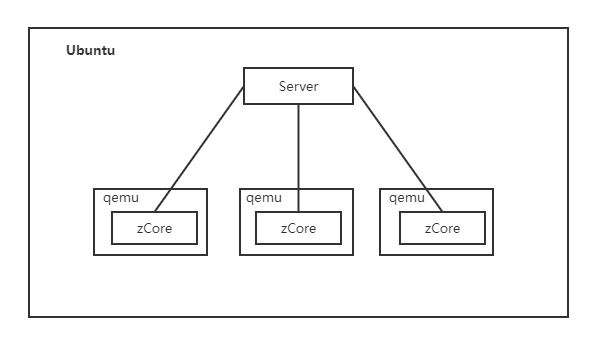
\includegraphics[width=\textwidth]{./images/image1.png}
\end{figure}
\end{frame}

\begin{frame}
\frametitle{Distributed Filesystem}
\framesubtitle{Future works}
  \begin{itemize}
    \item address consistency issues with locking primitives
    \item implement more fileystem operations
    \item automatic rebalance and migration of blocks
  \end{itemize}
\end{frame}

\section{}
\frame{\titlepage}
\end{document}
